
\section{System Setup}

\begin{figure}[h]
  \centering
  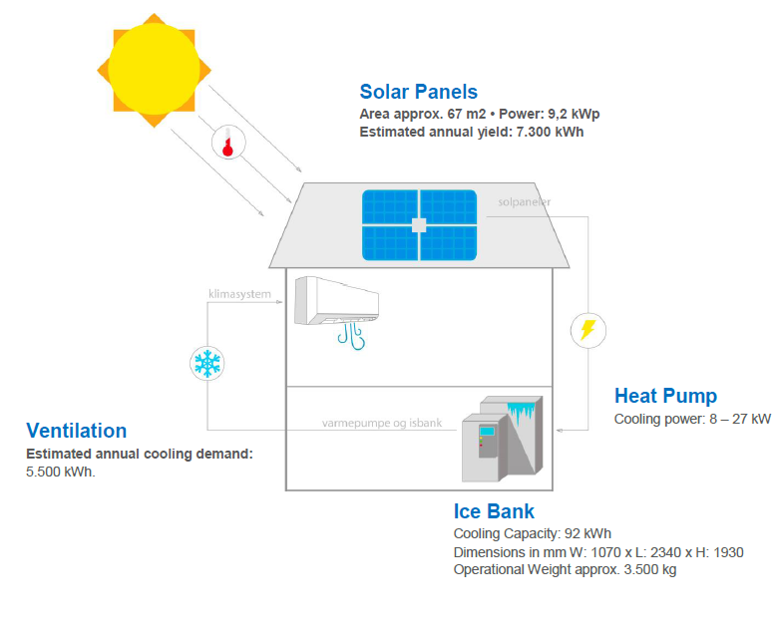
\includegraphics[scale=0.7]{figures/systemSetup}
  \caption{System Setup}
  \label{fig:systemSetup}
\end{figure}

\newpage
\section{State Space Representation}

\begin{align*}
  \frac{d}{dt}\statevec(t) &= A\statevec(t) + B\inputvec(t)
\end{align*}

Where:
\begin{itemize}
\item $\statevec$ is the state vector
\item $\inputvec$ is the input vector
\item $A$ is the state matrix
\item $B$ is the input matrix
\end{itemize}



\subsubsection{State Variables}

\begin{itemize}
\item
  $\troom$ the temperature of the room in \si{\degreeCelsius}
\item
  $\lib$ the level of the ice bank in in \si{\joule}
\item
  $\energyCom$ the energy consumption of the system in \si{\joule}
\item
  $\energySaved$ the energy saved by using solar panels in \si{\joule}
\item
  $\cost$ the total cost in \si{\dkk}
\end{itemize}

\subsubsection{Constants}
\begin{itemize}
\item $\cJtoC$ a constant mapping how power transfers to temperature
  in \si{\degreeCelsius\per\joule}
\item $\cri$ a constant indicating room insulation in
  \si{\degreeCelsius\per\degreeCelsius\per\second}
\item $\cir$ a constant indicating how irrandiance affects room 
  \si{\degreeCelsius\per\degreeCelsius\per\second}
\item $\ulib$ a constant indicating the maximal capacity of the ice bank
  \si{\joule}
\item $\llib$ a constant indicating the mininal allowed capacity of
  the ice bank \si{\joule}
\end{itemize}


\subsubsection{Input Variables}
\begin{itemize}
\item
  % [per-mode=fraction]
  $\irradiance$ the irradiance in \si{\watt\per\square\metre}
\item $\pump$ the setting of the pump in \si{\watt}
\item $\energys$ is the energy currently been saved in \si{\watt}
  which is computed as $\min(\pump,\irradiancesp)$ where
  $\irradiancesp$ the energy produced by the solar panel in \si{\watt}
\item
  $\tenv$ the outside temperature in \si{\degreeCelsius}
\item
  $\ventilator$ the amount of energy taken from the ventilator in \si{\watt}
\item $\pumpef$ the effective cooling power of the pump in \si{\watt}
\item $\costPerSecond$ the cost per second in \si{\dkk\per\second}
  computed as $\max(0,\costPerJoule\cdot(\pump - \irradiancesp))$
  where $\costPerJoule$ is the cost per joule in \si{\dkk\per\joule}.
  % \item $\cop$ the coefficient of performance of the pump given the
  %   speed of the pump in \si{\joule\per\joule}
  % \item
  %   $\cop_{\lib}$
  %   \[
  %     \cop_{\lib} =
  %     \begin{cases}
  %       0 & \text{ if } \lib > \ulib
  %       \\
  %       \cop & \text{ otherwise } 
  %     \end{cases}
  %   \]
\end{itemize}




\subsubsection{Differential Equations}

\[
  \begin{array}{rcl}
    \frac{d}{dt}\troom(t) &=& \cJtoC\cdot\ventilator + \cri\cdot(\tenv-\troom) + \cir\cdot\irradiance 
    \\[0.1cm]
    \frac{d}{dt}\lib(t) &=&  \pumpef - \ventilator
    \\[0.1cm]
    \frac{d}{dt}\energyCom(t) &=&  \pump
    \\[0.1cm]
    \frac{d}{dt}\energySaved(t) &=&  \energys
    \\[0.1cm]
    \frac{d}{dt}\cost(t) &=&  \costPerSecond
  \end{array}
\]

\subsection{Matrix Representation}




$A = 
\begin{bmatrix}
  -\cri & 0 & 0 & 0 & 0\\
  0 & 0 & 0 & 0 & 0\\
  0 & 0 & 0 & 0 & 0\\
  0 & 0 & 0 & 0 & 0\\
  0 & 0 & 0 & 0 & 0
\end{bmatrix},
\statevec =
\begin{bmatrix}
  \troom \\
  \lib\\
  \energyCom\\
  \energySaved\\
  \cost
\end{bmatrix},
B = 
\begin{bmatrix}
  \cir & 0 & 0 & \cri & \cJtoC & 0 & 0\\
  0 & 0 & 0 & 0 & -1 & 1 & 0\\
  0 & 1 & 0 & 0 & 0 & 0 & 0\\
  0 & 0 & 1 & 0 & 0 & 0 & 0\\
  0 & 0 & 0 & 0 & 0 & 0 & 1
\end{bmatrix},
\inputvec =
\begin{bmatrix}
  \irradiance\\
  \pump\\
  \energys\\
  \tenv\\
  \ventilator\\
  \pumpef\\
  \costPerSecond
\end{bmatrix}
$

\subsection{Built in Controllers}

\subsubsection{Pump Controller}
\begin{enumerate}
\item
  if $\lib \leq \llib$ then $\pump$ goes to its maximal
  setting
\item
  if $\lib \geq \ulib$ then $\pump$ is 0
\item
  else do not change the setting
\end{enumerate}

\subsubsection{Ventilation Controller}
Constants:
\begin{itemize}
\item
  $\tset$ is the temperature set point for the room
\item
  $\tsetdelta$ is the allowed margin of deviation from $\tset$
\end{itemize}

Controller:
\begin{enumerate}
\item
  if $\troom > (\tset + \tsetdelta)$ then $\ventilator$ is on
\item
  if $\troom < (\tset - \tsetdelta)$ then $\ventilator$ is off
\item
  else do not change the setting
\end{enumerate}

\section{UPPAAL Model}
See Figure \ref{fig:uppaal_model}.
\begin{itemize}
  \item $s$ is the current pump setting, $s \in \{0, 5000, 11000\}$ (off, mid, high)
	\item $control\_interval =$ 15 minutes $(60 \cdot 15)$
	\item $update\_state(s)$ solves the differential equations numerically
\end{itemize}
Input data from Matlab:

\begin{itemize}
	\item $\troom$
	\item $\lib$
	\item $\tenv, \irradiance$ and $\costPerJoule$\footnote{actually the cost of MWh, not Joule} in 15 minute intervals
\end{itemize}
\begin{figure}[htb]
	\centering
		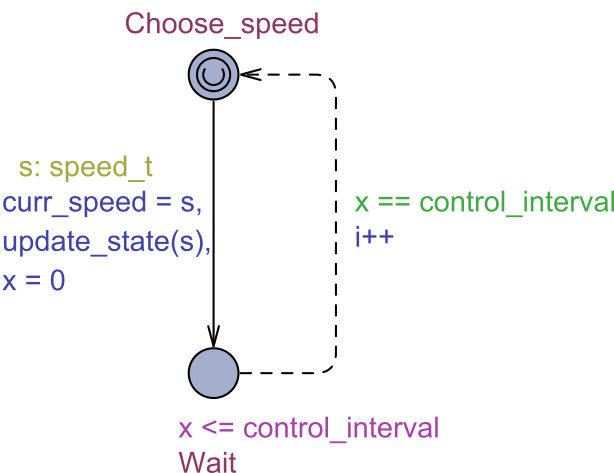
\includegraphics[scale=0.5]{figures/uppaal_model.png}
	\caption{UPPAAL Icebank Model}
	\label{fig:uppaal_model}
\end{figure}

\subsection{Stratego Controller}
\begin{verbatim}
strategy Opt = minE (C) [<=timeHorizon]: <> y >= timeHorizon
simulate 1 [<=timeHorizon] {curr_speed} under Opt
\end{verbatim}

\subsection{Na\"ive Controller}
\begin{itemize}
	\item Tries to match the generated energy by solar panels with one of the three pump settings.
\end{itemize}
The output speed is given by $\min_i d_i$ where

\[
D = \begin{bmatrix}
    |0-\irradiancesp|\\
		|5000-\irradiancesp|\\
		|11000-\irradiancesp|
    \end{bmatrix}
\]

\section{Data}

Weather data:
\begin{itemize}
	\item 2001 - 2010 Danish Design Reference Year (DRY)\footnote{http://www.dmi.dk/laer-om/generelt/dmi-publikationer/tekniske-rapporter/\\No. 13-19}
	\begin{itemize}
		\item A ``typical year'' in Denmark
		\item Temperature and irradiance 
		\item Hourly
  \end{itemize}	
\end{itemize}


Pricing data:
\begin{itemize}
	\item Historical electricity spot prices from Nord Pool\footnote{https://www.nordpoolgroup.com/historical-market-data/ \\Updates each day. DK1 $\approx$ Jutland+Funen. DK2 $\approx$ Zealand.}
	\item DKK/MWh
	\item Hourly
	\item Negative numbers
\end{itemize}








%%% Local Variables:
%%% mode: latex
%%% TeX-master: "../main.tex"
%%% End:
